\section{Methods and materials}\label{chap:methodsandmaterials}

This chapter will present a description of what and how this work will be done, as well as the tools and methods used. First ~\autoref{chap:methodsandmaterials:architecture} presents an overview of the architecture and how the proposed experiment will be done. Then, the ~\autoref{chap:methodsandmaterials:datasets} presents the datasets that will be used in the evaluation process. Finally in the ~\autoref{chap:methodsandmaterials:evaluation}, is shown how the evaluation will be done.

\subsection{Architecture overview}\label{chap:methodsandmaterials:architecture}

The proposed work basically consists of comparing different similarity techniques. Therefore, ~\autoref{fig:arq} defines an overview of the architecture with the intention of comparing several techniques using different features and testing them with two datasets.

\begin{figure}[h]
	\caption{Proposed architecture}
	\label{fig:arq}
	\centering%
	\begin{minipage}{.8\textwidth}
		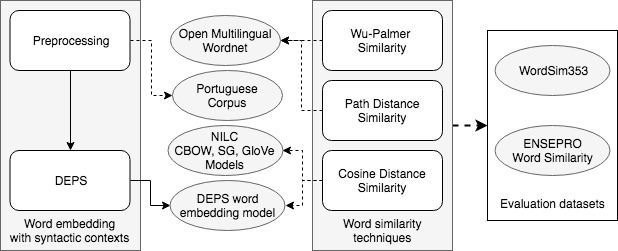
\includegraphics[width=\textwidth]{arq.jpg}
		\fonte{Made by the author.}
	\end{minipage}
\end{figure}

In this model will be compared techniques based on lexical bases, in this case, Open Multilingual Wordnet (OMW) will be used with Path Distance and Wu-Palmer similarity techniques. It was decided to use OMW due to its ease of use through the Natural Language Toolkit (NLTK) library available for the Python programming language as well as the availability of the Portuguese language for querying the synsets.

In the distributional approach it will be used pre-trained models of word embeddings available by Núcleo Interinstitucional de Linguística Computacional (NILC) in different implementations, being CBOW, SG, and GloVe. Also available, there are pre-trained models with different dimensions being 50, 100, 300, 600 and 1000. But initially I will use the models of 300 dimensions and if it is necessary, I will experiment with different values. The metric to be used for the comparison of similarity between one word and another will be the cosine distance.

One of the main tasks in this work is to take into account the syntactic tree information of the sentences in a Portuguese corpus to train the word embeddings. And for this, the algorithm implementation by \citetext{Levy2014} will be used. This will result in a new word embedding model in which the evaluation will be performed in the same way that the NILC word embeddings were covered. PALAVRAS syntactic parser is intended to be used for the annotation of the corpus with syntactic information.

\subsection{Datasets}\label{chap:methodsandmaterials:datasets}

\subsubsection{WordSimilarity-353 Test Collection}

The WordSimilarity-353 is a test collection for measuring word similarity developed by \citetexto{Finkelstein:2001:PSC:371920.372094}. This dataset contains two sets of English word pairs along with human-assigned similarity judgements.

% http://www.cs.technion.ac.il/~gabr/resources/data/wordsim353/

\subsubsection{ENSEPRO Word Similarity}

Aiming to prove an improvement in the accuracy of information extraction systems, a specific dataset will be assembled using the questions and answers of short sentences used in the ENSEPRO system. This system evaluation was made using the dataset for the challenge Question Answering over Linked Data (QALD-7) of 2017, which also had the addition of the Portuguese language. For each sentence of the Portuguese questions of this dataset, we will assemble a new dataset with only the keywords necessary to carry out queries via the ENSEPRO search engine. A pair of this keyword must be generated with the one that is currently in the linked data. For words that the system currently cannot find answers due to lack of a word in the expansion of related terms, it will be investigated manually which would be the word that should be found and added to the dataset. Also, the dataset will include the syntactic information for each keyword.

\subsection{Evaluation}\label{chap:methodsandmaterials:evaluation}

For the evaluation, we propose to do qualitative measure based on a manual inspection of the most similar words to a hand picked set of words and see if they are in fact similar or not to the other words regarding similarity, relatedness and also the syntactic similarity.
Also a quantitative analyses is proposed by using the WordSim353 dataset from \citetexto{Finkelstein:2001:PSC:371920.372094}, which is a dataset regarding word similarity versus relatedness. As all the pairs in this dataset are in English, they will be manually translated to Portuguese to be able to compare the results with all the techniques.
To better visualize the performance of each technique the precision-recall curve draws will be used to describes the embeddings affinity.
Another quantitative analysis will be done to see if the recall increase using the ENSEPRO dataset. If it increases it will improve the quality of the ENSEPRO system. 







% CÓDIGO: https://levyomer.wordpress.com/2014/04/25/dependency-based-word-embeddings/
% DATASET: http://www.cs.technion.ac.il/~gabr/resources/data/wordsim353/

% resources:
% - Open Multilingual Wordnet
% - NILC Pre-trained word embeddings models
% Corpus:
%  - Pegar com o allan o corpus portugues
%  - Anotar o corpus com o PALAVRAS syntactic parser
% quantitative evaluation datasets:
%  - WordSim353 manual translation to portuguese
%  - ENSEPRO word similarity (vou criar em conjunto com o denis, preciso definir formato e como, usando as perguntas do QALD)
% Algoritmo:
%  - Usar o código fonte do DEPS
% tools:
%  - Palavras
%  - Python NLTK, word2vec, word2vecf, 













% \begin{itemize}
%     \item Explore the existing techniques regarding word similarity, using a distributional approach called word embeddings, adapting existing works to Brazilian Portuguese.
%     \item Compare the word embeddings approach to other techniques that are solely based on a lexical database such as WordNet.
%     \item Adapt existing studies regarding the addition of syntactic context in the training process of word embeddings to a Brazilian Portuguese corpus, to check if the results will be, similar or not. 
%     \item Evaluate the different techniques over a common \textit{dataset} related to \citetexto{denis2018} work.
% \end{itemize}

% This thesis is structured as follows. The \autoref{chap:background} presents the general concepts and techniques used in this work. In \autoref{chap:relatedwork} are described and analyzed the works related to the research area of this work. The \autoref{chap:methodsandmaterials} presents the proposed model, as well as the form of the experiment and the necessary tools. The \autoref{chap:results} presents the preliminary results obtained in the case study experiment. Finally, \autoref{chap:conclusions} summarizes the thesis findings, contributions, and discusses.





% Descrever um cenário em que o projeto se faz necessário (Extração de informação em ontologias utilizando Linguagem Natural - Talvez citar o uso de queries que utilizem triplas RDF) e ajuda a resolver o problema. Após descrito citar como exemplo o trabalho do denis e detalhar o cenário dele.

% - Cenário do denis: Recebe uma pergunta; Realiza um parse, extraindo palavras relevantes e seu contexto sintático; Realiza a geração de combinações diferentes de possíveis tuplas RDF de pesquisa; Algumas dessas pesquisas não se encontra a resposta, porém se uma destes elementos da tupla fosse substituído por um outro sinônimo ele iria encontrar a resposta. Portanto é usado o WordNet BR para procurar por sinônimos, porém ainda assim, nem sempre se tem a palavra cadastrada no WordNet.

% Descrever a arquitetura do modelo proposto.

% - Usar o NLTK python e procurar por sinônimos de uma dada palavra no OpenWordNet-PT ( supõe-se que algumas vezes não será encontrado nada )
% - Usar diferentes tipos de word embedding (BoW, SG, GloVe)
% - [TCC2]Treinar word embeddings sobre um corpus (pegar com o allan) utilizando o contexto gerado pelo POS Tagger da unisinos (Aonde consigo??)
% - [TCC2]Algum outro algoritmo se houver necessidade
% - Testar cada abordagem com o dataset do denis




% OpenWordNet-PT. \cite{coling2012}.

